\documentclass{article}

\usepackage[margin=1in]{geometry}
\usepackage{graphicx} % Allow image/pdf includes
\usepackage{extramarks} % Extra header marks (continued on next page)
\usepackage{amsmath} % Math enhancements
\usepackage{amsthm} % Theorem typesetting
\usepackage{amssymb} % Extended symbol collection
\usepackage{tikz} % Graphical element creation
\usetikzlibrary{automata,positioning}
\usepackage{algpseudocode} % Algorithm layout
\usepackage{enumitem} % Enumerate (lists)
\usepackage{ragged2e} % Alternative alignment
\usepackage{gensymb} % Generic symbols (degree, etc)
\usepackage{empheq} % Allow \boxed around \begin{empheq}
\usepackage{color,soul} % Highlighting
\usepackage{booktabs} % Enhanced table creation
\usepackage{multirow} % Table multi row
\usepackage{mathtools} % Math enhancements
\usepackage{bm} % Bold math
\usepackage[mathscr]{euscript} % Script variables
\usepackage{cancel} % Cancel through text
\usepackage{color,soul} % Highlighting
\usepackage{mathtools}
\usepackage{multirow}
\usepackage{mathrsfs}
\usepackage{physics}
\usepackage{gensymb}
\usepackage{siunitx}
\usepackage{subcaption}
\usepackage[]{algorithm2e}
\usepackage{float}
\usepackage[T1]{fontenc}
\usepackage{diagbox}
\usepackage{stmaryrd}
\usepackage[numbers]{natbib}
\usepackage{booktabs}

\setlength\parindent{0pt} % No indents
\setlength{\parskip}{1em} % Paragraph skip

\newcommand{\vx}{\mathbf{x}} % x vector
\newcommand{\vo}{\mathbf{\Omega}} % omega vector
\newcommand{\vn}{\mathbf{n}} % normal vector
\newcommand{\spatial}{\mathcal{D}} % spatial domain representation
\newcommand{\boundary}{\delta \mathcal{D}} % boundary representation
\newcommand{\angular}{\mathcal{S}} % angular domain representation
\DeclarePairedDelimiterX{\ainp}[2]{\langle}{\rangle}{#1, #2}
\newcommand{\pinp}[2]{\left(#1,#2\right)}

\newcommand{\pageTitle}{MATH 676 -- Final Report}
\newcommand{\pageAuthor}{Logan Harbour}

\begin{document}

\title{\LARGE \textbf{\pageTitle} \vspace{-0.3cm}}
\author{\large \pageAuthor}
\date{\vspace{-0.6cm} \large \today \vspace{-0.4cm}}

\maketitle

\section{Introduction}

The majority of my dissertation is to involve acceleration for method of characteristics (MOC) radiation transport. Many acceleration methods for discrete ordinates (S$_N$) radiation transport are similar to those utilized in MOC transport. Therefore, my overarching goal for this course was to investigate and implement common acceleration methods for S$_N$ transport utilizing Deal.ii. In specific, the focus is on diffusion synthetic acceleration (DSA) of source iteration \cite{adams2002fast} in discrete ordinates radiation transport.

With source iteration (see Section \ref{subsec:SI}), the scattering term is lagged. For example, one first solves for the solution of particles that have not scattered. These particles are then used to determine the source of first-scattered particles, and so on. The issue lies in the fact that when the ratio of particles scattering to being absorbed is close to unity, the source iteration process requires a significant number of iterations. DSA is able to attenuate the most poorly attenuated errors very well, therefore the diffusion problem is used as a corrector to the scalar flux after each source iteration.

From this, the primary goals of this work are as follows:
\begin{enumerate}
	\item Develop a one-group, discrete ordinates radiation transport code in Deal.ii
	\item Develop a one-group, diffusion radiation transport code in Deal.ii
	\item Utilize the diffusion code to estimate the error after a source iteration as a preconditioner
\end{enumerate}

The primary goals were completed approximately a month before the deliverables for the course were due. Therefore, the following additional implementations were made:
\begin{enumerate}
	\item Parallel support using the Trilinos wrappers
	\item Reflecting boundary conditions, which require additional iteration within a source iteration
	\item Acceleration of reflecting boundary conditions within the DSA solver
\end{enumerate}

\section{Methods}

Begin with the spatial domain $\spatial \in \mathbb{R}^2$ in which $\boundary$ is on the boundary of $\spatial$. The set of propagation directions $\angular$ is the unit disk.

The linear Boltzmann equation for one-group transport is
\begin{subequations}
	\label{eq:boltzmann}
	\begin{equation}
	\vo \cdot \nabla \Psi(\vo, \vx) + \sigma_t(\vx) \Psi(\vo, \vx) - \sigma_s(\vx) \Phi(\vx) = q(\vx)\,, \qquad \forall (\vo, \vx) \in \angular \times \spatial\,,
	\end{equation}
	\begin{equation}
	\Phi(\vo, \vx) = \Phi^\text{inc} (\vo, \vx)\,, \qquad \forall(\vo, \vx) \in \angular \times \boundary\,,~ \vo \cdot \vn(\vx) < 0\,,
	\end{equation}
\end{subequations}
where $\Phi$ is the scalar flux, defined by
\[
\Phi = \frac{1}{2\pi} \int_{\angular} \Phi(\vo, \vx) d\Omega\,.
\]

Define $\mathbb{T}_h$ as the set of all active cells of the triangulation for $\spatial$ and $\mathbb{F}_h$ as the set of all active interior faces and define a discontinuous approximation space for the scalar flux based on the mesh $\mathbb{T}_h$ as
\begin{equation}
	V_h \in \{ v \in L^2(\spatial)~|~\forall K \in \mathbb{T}_h\,, v|_K \in P_K\}\,,
\end{equation}
where the finite-dimensional space $P_K$ is assumed to contain $\mathbb{P}_k$, the set of polynomials of degree at most $k$. Denote interior edges as $\mathcal{E}_h^i$ and boundary edges as $\mathcal{E}_h^b$. 

\subsection{S$_N$ discretization}

Introduce the S$_N$ discretization, which replaces the angular flux with a discrete angular flux, as
\begin{equation}
\label{eq:sn_discretization}
\psi(\vx) = [\psi_1(\vx), \psi_2(\vx), \ldots \psi_{N_\Omega}(\vx)]^T\,.
\end{equation}
We then introduce the quadrature rule $\{ (\vo_d, \omega_d), d = 1, \ldots, N_\Omega\}$ where $\sum_d \omega_d = 1$. With said quadrature rule, we have 
\[
\int_\angular f(\vo, \vx) d\Omega \approx \sum_{d = 1}^{N_\Omega} w_d f(\vo_d, \vx)\,.
\]
This discretization allows us to write the system in Equation \eqref{eq:boltzmann} as
\begin{subequations}
	\label{eq:sn_equations}
	\begin{equation}
	\label{eq:sn_equations_domain}
	\vo_d \cdot \nabla \psi_d(\vx) + \sigma_t(\vx) \psi_d(\vx) - \sigma_s(\vx) \phi(\vx) = q(\vx)\,, \qquad \forall \vx \in \spatial
	\end{equation}
	\begin{equation}
	\label{eq:sn_equations_boundary}
	\psi_d(\vx) = \Psi^\text{inc}_d (\vx)\,, \qquad \forall \vx \in \boundary\,,~ \vo_d \cdot \vn(\vx) < 0\,, 
	\end{equation}
\end{subequations}
where the discrete scalar flux, $\phi$, is
\[
	\phi(\vx) =  \sum_{d = 1}^{N_\Omega} w_j \psi_j(\vx)\,.
\]

To obtain the weak form, multiply Equation \eqref{eq:sn_equations_boundary} by the test function $v_d \in V_h$ and integrate as
\begin{equation}
	\int_{\mathbb{T}_h} \vo_d \cdot \nabla \psi_d v_d + \int_{\mathbb{T}_h} \sigma_t \psi_d v_d - \int_{\mathbb{T}_h} \sigma_s \phi v_d = \int_{\mathbb{T}_h} qv_d\,,
\end{equation}
and integrate the first term by parts to obtain
\begin{equation}
	\label{eq:sn_fem_parts}
	\int_{\mathbb{T}_h} -\vo_d \cdot \nabla v_d\psi_d + \int_{\mathcal{E}_h^i} \psi_d (\vo_d \cdot \vn) v_d + \int_{\mathbb{T}_h} \sigma_t \psi_d v_d - \int_{\mathbb{T}_h} \sigma_s \phi v_d = \int_{\mathbb{T}_h} qv_d\,,
\end{equation}
where $\vn$ is the outward normal. Note that the surface integration in Equation \eqref{eq:sn_fem_parts} is double-valued due to the discontinuous approximation. We introduce the upwind approximation
\begin{equation}
	\psi_d \vo_d \cdot \vn = \psi^+_d \vo_d \cdot \vn\,,
\end{equation}
where $\psi_d^+$ is the upwind value of $\psi_d$, that is, the value from the side of the face in which $\vo \cdot \vn \geq 0$. The weak form is then defined as
\begin{equation}
	\label{eq:sn_fem_upwind}
	\int_{\mathbb{T}_h} -\vo_d \cdot \nabla v_d\psi_d + \int_{\mathcal{E}_h^i} \psi_d^+ (\vo_d \cdot \vn) v_d + \int_{\mathbb{T}_h} \sigma_t \psi_d v_d - \int_{\mathbb{T}_h} \sigma_s \phi v_d = \int_{\mathbb{T}_h} qv_d\,.
\end{equation}

\subsection{Source iteration}
\label{subsec:SI}

To converge the scattering source, cast Equation \eqref{eq:sn_equations_domain} with iterative index $\ell$ as
\begin{equation}
	\label{eq:si}
\vo_d \cdot \nabla \psi_d^{(\ell + 1)} + \sigma_t \psi_d^{(\ell + 1)} = \sigma_s \phi^{(\ell)} + q\,,
\end{equation}
with $\psi_d^{(0)} = \phi^{(0)} = \vec{0}$. After solving each direction, $d$, for an iteration $\ell$ in Equation \eqref{eq:si}, update the scalar flux with
\begin{equation}
	\label{eq:si_update}
	\psi^{(\ell + 1)} = \sum_{d = 1}^{N_\Omega} w_d \psi_d^{(\ell + 1)}\,.
\end{equation}
The process is then to be repeated until $\left\lVert\phi^{(\ell + 1)} - \phi^{(\ell)}\right\rVert_{L^2} < \tau$, where $\tau$ is some tolerance, typically $10^{-12}$. $\psi^{(\ell + 1)}$ is the particles that have scattered at most $\ell$ times. As $\sigma_s / \sigma_t \to 1$, particles scatter more and more before they are absorbed and the number of needed source iterations becomes significant.

\subsection{Diffusion acceleration}

Simple algebraic manipulations can show that the error in $\psi^{(\ell + 1)}$ satisfies the same transport equation with a source equal to $R^{(\ell + 1)} = \sigma_s (\psi^{(\ell + 1)} - \psi^{(\ell)})$. Furthermore, a Fourier analysis shows that the transport equation with the diffusion approximation attenuates the errors most poorly attenuated by the transport sweep. Therefore, we will cast a diffusion problem with the previously defined source as a preconditioner to source iteration.
	
Consider then the approximated error in $\psi^{(\ell + 1)}$, defined as $e^{(\ell + 1)}$. The corresponding diffusion problem is
\begin{equation}
	\label{eq:diffusion}
	- \nabla \cdot D \nabla e^{(\ell + 1)} + \sigma_a e^{(\ell + 1)} = \sigma_s (\phi^{(\ell + 1)} - \phi^{(\ell)})\,,
\end{equation}
where $D$ is the diffusion coefficient, $D = 1 / 3 \sigma_t$.

Cast Equation \eqref{eq:diffusion} in the same DG space with interior edges $\mathcal{E}_h^i$ and boundary edges $\mathcal{E}_h^b$ using a modified interior penalty method developed in \cite{ragusa2010two} for the face terms to obtain
\begin{multline}
	\int_{\mathbb{T}_h} (D \nabla e^{(\ell + 1)} \cdot \nabla v + \sigma_a e^{(\ell + 1)} v) + \int_{\mathcal{E}_h^i} \left( \{\!\!\{ D \delta_n e^{(\ell + 1)} \}\!\!\} \llbracket v \rrbracket + \{\!\!\{ D \delta_n v \}\!\!\} \llbracket e^{(\ell + 1)} \rrbracket + \kappa \llbracket e^{(\ell + 1)} \rrbracket \llbracket v \rrbracket \right) \\
	+ \int_{\mathcal{E}_h^b} \left( \kappa e^{(\ell + 1)} v - D v \delta_n e^{(\ell + 1)} - D e^{(\ell + 1)} \delta_n v \right) = \int_{\mathbb{T}_h} \sigma_s (\phi^{(\ell + 1)} - \phi^{(\ell)}) v\,,
\end{multline}
	where
\[
	\{\!\!\{ u \}\!\!\} \equiv \frac{u^+ + u^-}{2} \quad \text{and} \quad \llbracket u \rrbracket \equiv u^+ - u^-\,,
\]
in which the penalty coefficient is
\[
	\kappa = \begin{cases} 2 \left(\frac{D^+}{h^+_\bot} + \frac{D^-}{h^-_\bot}\right) & \text{for~interior~edges}\,, \\ 8 \frac{D^-}{h^-_\bot} & \text{for~boundary~edges}\,, \end{cases}
\]
and $h^\pm_\bot$ is a characteristic length of the cell in the direction orthogonal to the edge.

\section{Code design and description}

The bulk of the development resides in five classes, of which the \texttt{Problem} owns an instance of the other four. There are no public variables and the only access to private variables is through appropriately created getter methods that ensure const-correctness when possible. All primary system (LHS, RHS, solution) storage is done using the Deal.ii wrappers for the Trilinos vector and sparse matrix. A summary of these five classes follows in the next subsections. 

\subsection{\texttt{Description} class}

The \texttt{Description} class stores all of the materials and boundary conditions in the problem. It does not need access to any of the other classes as this information is initialized once at setup by the \texttt{Problem} and only read from \texttt{SNProblem} and \texttt{DSAProblem} during assembly. Its \texttt{setup\_bcs()} and \texttt{setup\_materials()} methods require access to a set of boundary and material ids, respectively, in order to confirm that total material and boundary condition coverage is provided.

The interface to materials and boundary conditions is provided to the other classes by the public methods \texttt{get\_bc()} and \texttt{get\_material()}, which return a reference to the custom \texttt{BC} and \texttt{Material} structs, respectively.

\subsection{\texttt{Discretization} class}

The \texttt{Discretization} class is storage for all that pertains to the triangulation and the degree of freedom handler. In specific, it generates the mesh (depending on user input), builds the degree of freedom handler, and distributes the degrees of freedom, builds the sparsity pattern, etc. It also builds the custom \texttt{AngularQuadrature} object, which contains the angular quadrature. The two classes that assemble and solve the problems, the \texttt{SNProblem} and \texttt{DSAProblem} have read-only access to some of the variables in the \texttt{Discretization}; namely the \texttt{DoFHandler}. Lastly, it also builds the listing of all boundary and material ids for use in verifying material and boundary condition coverage by the \texttt{Description}.

\subsection{\texttt{Problem} class}

As stated in the beginning of the section, the \texttt{Problem} stores instances of all of the classes that are discussed here. It stores the system matrix, system right hand side, solution vectors, and other data structures that are needed by both the \texttt{DSAProblem} and \texttt{SNProblem}. It stores the primary \texttt{solve()} method, which iterates and checks for convergence of the \texttt{DSAProblem} and \texttt{SNProblem} as needed. Lastly, it stores the \texttt{.vtu} output if requested via input.

\subsection{\texttt{SNProblem} class}

The \texttt{SNProblem} class assembles and solves the S$_N$ problem. It does not interface with the \texttt{DSAProblem} at all, purposely chosen in the design. Its public method available to the \texttt{Problem} is \texttt{assemble\_solve\_update()}, which assembles, solves, and updates the solution for all of the directions in the problem.

The assembly and solve process for a specific direction are handled in the private methods \texttt{solve()} and \texttt{assemble()}. The assembly process is handled by the \texttt{MeshWorker::loop()}, which calls on the private methods \texttt{integrate\_cell()}, \texttt{integrate\_boundary()} and \texttt{integrate\_face()} to integrate cells, boundaries, and interior faces, respectively. It is important to note that setting the \texttt{MeshWorker::LoopControl} \texttt{faces\_to\_ghost} parameter to \texttt{both} disables the need for communicating ghosted values of the system matrix. This is because the faces that are on ghosted cells are assembled on both sides of the processor boundary. The \texttt{solve()} method utilizes the Trilinos GMRES solver and AMG preconditioner.

The majority of the structure for the implementation of the \texttt{SNProblem} was provided by the Deal.ii step-12. The parallel implementation was derived from the Deal.ii step-40.

\subsection{\texttt{DSAProblem} class}

The \texttt{DSAProblem} class assembles and solves the diffusion problem utilized for acceleration of the S$_N$ source iterations. It does not interface with the \texttt{SNProblem} at all, purposely chosen in the design. Its public method available to the \texttt{Problem} is \texttt{assemble\_solve\_update()}, which assembles, solves, and updates the error estimate for the scalar flux error. 

At initialization, \texttt{assemble\_initial()} is called, which utilizes the \texttt{MeshWorker::loop()} to build the non-changing system matrix for the diffusion problem into the sparse matrix \texttt{dsa\_matrix}. This matrix is then to be utilized at the beginning of every full assembly step in \texttt{assemble()} in order to reduce the need to re-build every iteration.

The assembly and solve process for a single iteration are handled in the private methods \texttt{solve()} and \texttt{assemble()}. The assembly process is handled by the \texttt{MeshWorker::loop()}, which calls on the private methods \texttt{integrate\_cell()} and \texttt{integrate\_boundary()} to integrate cells and boundaries, respectively. The \texttt{solve()} method utilizes the Trilinos CG solver (the interior penalty method is symmetric) and AMG preconditioner.

The majority of the structure for the implementation of the \texttt{SNProblem} was provided by the Deal.ii step-12 and step-39. The parallel implementation was derived from the Deal.ii step-40.

\section{Numerical results}

\subsection{Constant solutions}

Take a problem with a domain of $[0, 10]^2$, $32^2$ elements, S$_2$ quadrature, a homogeneous volumetric source of $q = 1$, and $\sigma_t = 100$. The top and right boundary conditions are reflective and the bottom and left boundary vary. One would expect that the constant solution in the interior of the domain is $q / \sigma_a$. With this, we the following four problems:
\begin{itemize}
	\item $\sigma_s = 99$ and incident isotropic flux boundary conditions on the bottom and left of $q / \sigma_a$
	\item $\sigma_s = 99$ and vacuum boundary conditions on the bottom and left
	\item Without scattering and incident isotropic flux boundary conditions on the bottom and left of $q / \sigma_a$
	\item Without scattering and vacuum boundary conditions on the bottom and left
\end{itemize}

The inputs for these examples can be found in \texttt{examples/constant\_solution} and the results are plotted below in Figure \ref{fig:constant}.

\begin{figure}[H]
	\centering
	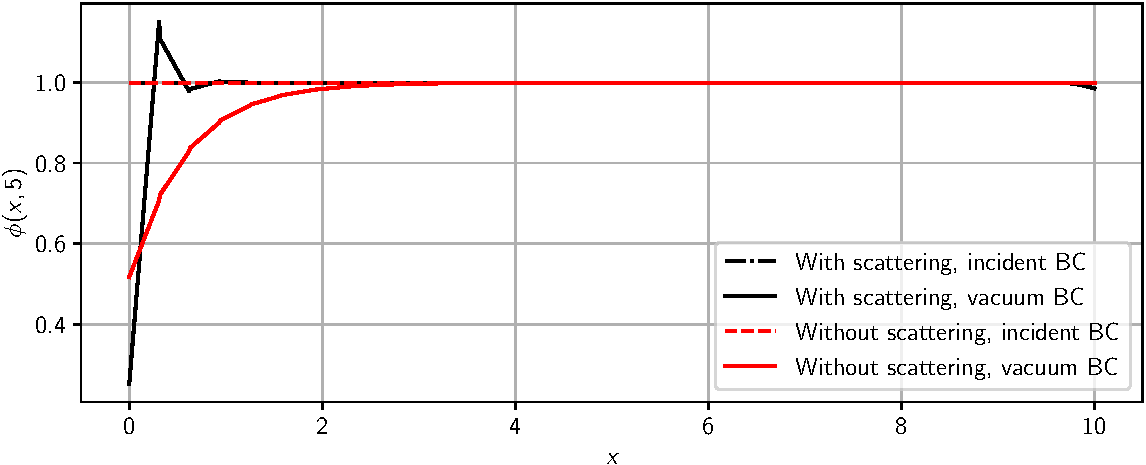
\includegraphics[width=0.9\linewidth]{images/constant_solution}
	\caption{The scalar flux along $y = 5$ for the constant solution problems.}
	\label{fig:constant}
\end{figure}

For the two cases with incident isotropic flux boundary conditions, as the flux condition is equal to the constant solution, we would expect the near the constant solution for the entire domain (as seen). For the case with scattering and vacuum boundary conditions, the cells are optically thick therefore we would expect a jump and drop at the vacuum boundary. For the case without scattering and vacuum boundary conditions, we would expect a decaying exponential to the constant solution. All of these features are seen. 

\subsection{DSA}

To verify the diffusion synthetic acceleration implementation, a problem was considered with increasing scattering ratio $c = \sigma_s / \sigma_t$. The spatial domain is $[0, 10]^2$, discretized into $16^2$ elements with S$_{10}$ angular quadrature. The cross sections are $\sigma_a + \sigma_s = \sigma_t = 100$ with a uniform volumetric source of 1. The input and run script are located in \texttt{examples/dsa\_convergence}. The $L_2$ norm of the difference in scalar flux was plotted with varying $c$, as seen below in Figure \ref{fig:dsa}.

\begin{figure}[H]
	\centering
	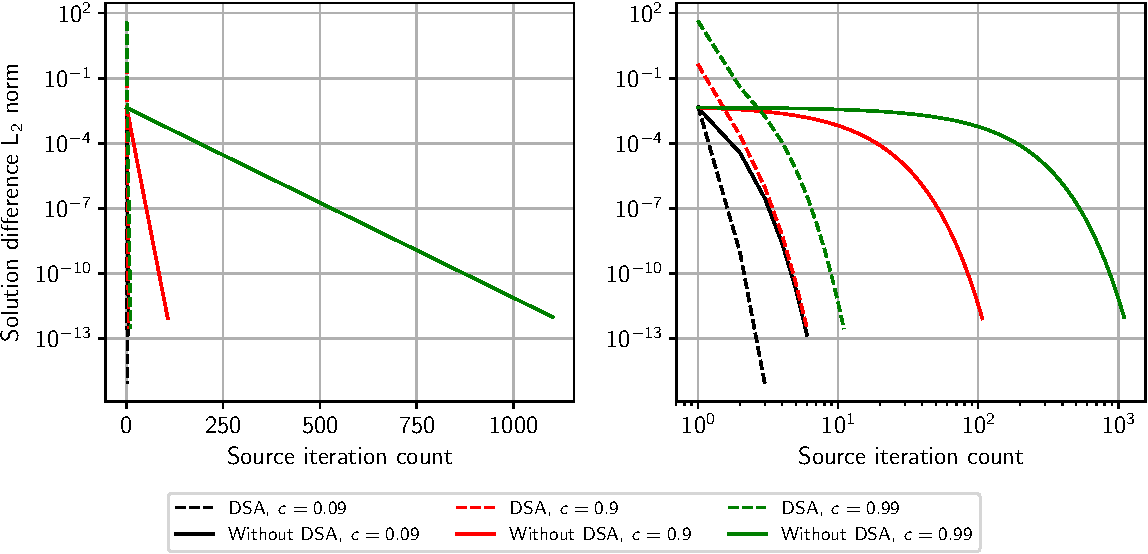
\includegraphics[width=0.9\linewidth]{images/dsa_residuals}
	\caption{Source iteration norms with and without diffusion acceleration.}
	\label{fig:dsa}
\end{figure}

\section{Conclusion}

The primary goals have been met for this project, and have shown successful results. Additional goals were created after reaching the primary goals early, and were also successful. I was very pleased to develop in Deal.ii and the code created for this project has shown to be a very successful test bed for other acceleration techniques. This is primarily due to the ease of development using Deal.ii and the \textit{plethora} of documentation available.

I have no doubt that both myself and my advisor will come to utilize this code again in the near future. A list of future works has already been developed for the coming months:
\begin{enumerate}
	\item Multi-group support
	\item Eigenvalue problem support
	\item Acceleration of eigenvalue problems using DSA
	\item Experimentation with other parallel solvers (pAIR!)
\end{enumerate}

\renewcommand\refname{References}
\bibliographystyle{unsrtnat}
\bibliography{ref} 

\end{document}

